	\documentclass[
    DIV12,
    cleardouble=plain,
    headings=normal,
    pdftex,
    headexclude,footexclude,
    final
]{scrreprt}


%\usepackage{spreadtab}
\usepackage{xspace}
\usepackage[ngerman]{babel}
\usepackage[utf8]{inputenc}
%\usepackage[T1]{fontenc}
\usepackage[pdftex]{graphicx}
\usepackage[bookmarks]{hyperref}
\usepackage{scrpage2}
\usepackage{longtable}
\usepackage{caption}
\usepackage{pgfplots}
\usepackage{float}
\usepackage{xcolor}
\usepackage{colortbl}
\usepackage{tabularx}
\usepackage{multirow} % tabelle
\usepackage{listings} % code aus datei einbinden
\usepackage{scrhack}
\usepackage{comment}


% word wrap with a red arrow
\lstset{
  basicstyle=\ttfamily,
  columns=fullflexible,
  frame=single,
  breaklines=true,
  postbreak=\mbox{\textcolor{red}{$\hookrightarrow$}\space},
}

\graphicspath{{./}{./images/}}

% #################################################################

\hyphenation{Cha-otn-gsch-werl}
\setlength\headheight{1.75cm}

\ihead{\small{Hochschule Hof}}
\chead{}
\ohead{
\includegraphics[height=0.05\textheight]{fh_logo}}
\pagestyle{scrheadings}


\setcounter{secnumdepth}{5}
\setcounter{tocdepth}{5}
\renewcommand{\arraystretch}{1}

\parskip0.5\baselineskip plus 0.125\baselineskip minus 0.25\baselineskip
\parindent0em

%\automark[section]{chapter}

\titlehead{\begin{center}
\includegraphics[width=5cm]{fh_logo}\end{center}}
 \title{
  Entwicklung einer Android Food Tracking App \\[1em]
  in der Programmiersprache Kotlin  
}
\publishers{Vorgelegt bei Prof. Dr. Michael Stepping}

\author{Johannes Franz, Normen Krug}


\date{Wintersemester 2017/2018}


\begin{document}
\maketitle


\pagenumbering{roman}

\tableofcontents

%\listoftables

\newpage
\pagenumbering{arabic}


\chapter{Einleitung}
Ziel ist es eine App zu entwickeln, die einen Rückschluss von sich zugenommener Nahrung auf Symptome zu ermöglichen. Dabei helfen die in der App eingetragenen Datenpunkte und Fotos diese mit einer z.B. allergischen Reaktion zu verknüpfen.
Zielgruppe sind dabei Menschen, die wegen Erkrankungen aus ihren zu sich zugenommenen Speisen und Getränken Rückschlüsse auf ihr Wohlbefinden treffen wollen.


\newpage

\chapter{Motivation}
Durch eigenen Bedarf motiviert entstand die Idee für diese App. Um aus wiederkehrenden Mahlzeiten eine Unverträglichkeit abzuleiten, stellt die App Funktionen bereit.



\chapter{Kotlin als Programmiersprache}
Für die App wurde die Programmiersprache Kotlin verwendet, welche auf der Google IO im Mai 2017 als offizielle Sprache für Android eingeführt wurde. Kotlin hat einen besser lesbaren Syntax als Java. 


\newpage

\chapter{Entwurfsphase}
In der Entwurfsphase wurde keine Zeit verschwendet und der Fokus auf Handskizzen gelegt. Da die Teammitglieder die zur Verfügung stehenden Steuerelemente in Android  Der unnötige Schritt diese in einem professionellen Entwurf nachzubauen sparte Zeit, so dass sich direkt mit der Programmierung beschäftigt werden konnte.

Erster Screen Entwurf:

\begin{figure}[ht]
	\centering
  \frame{ 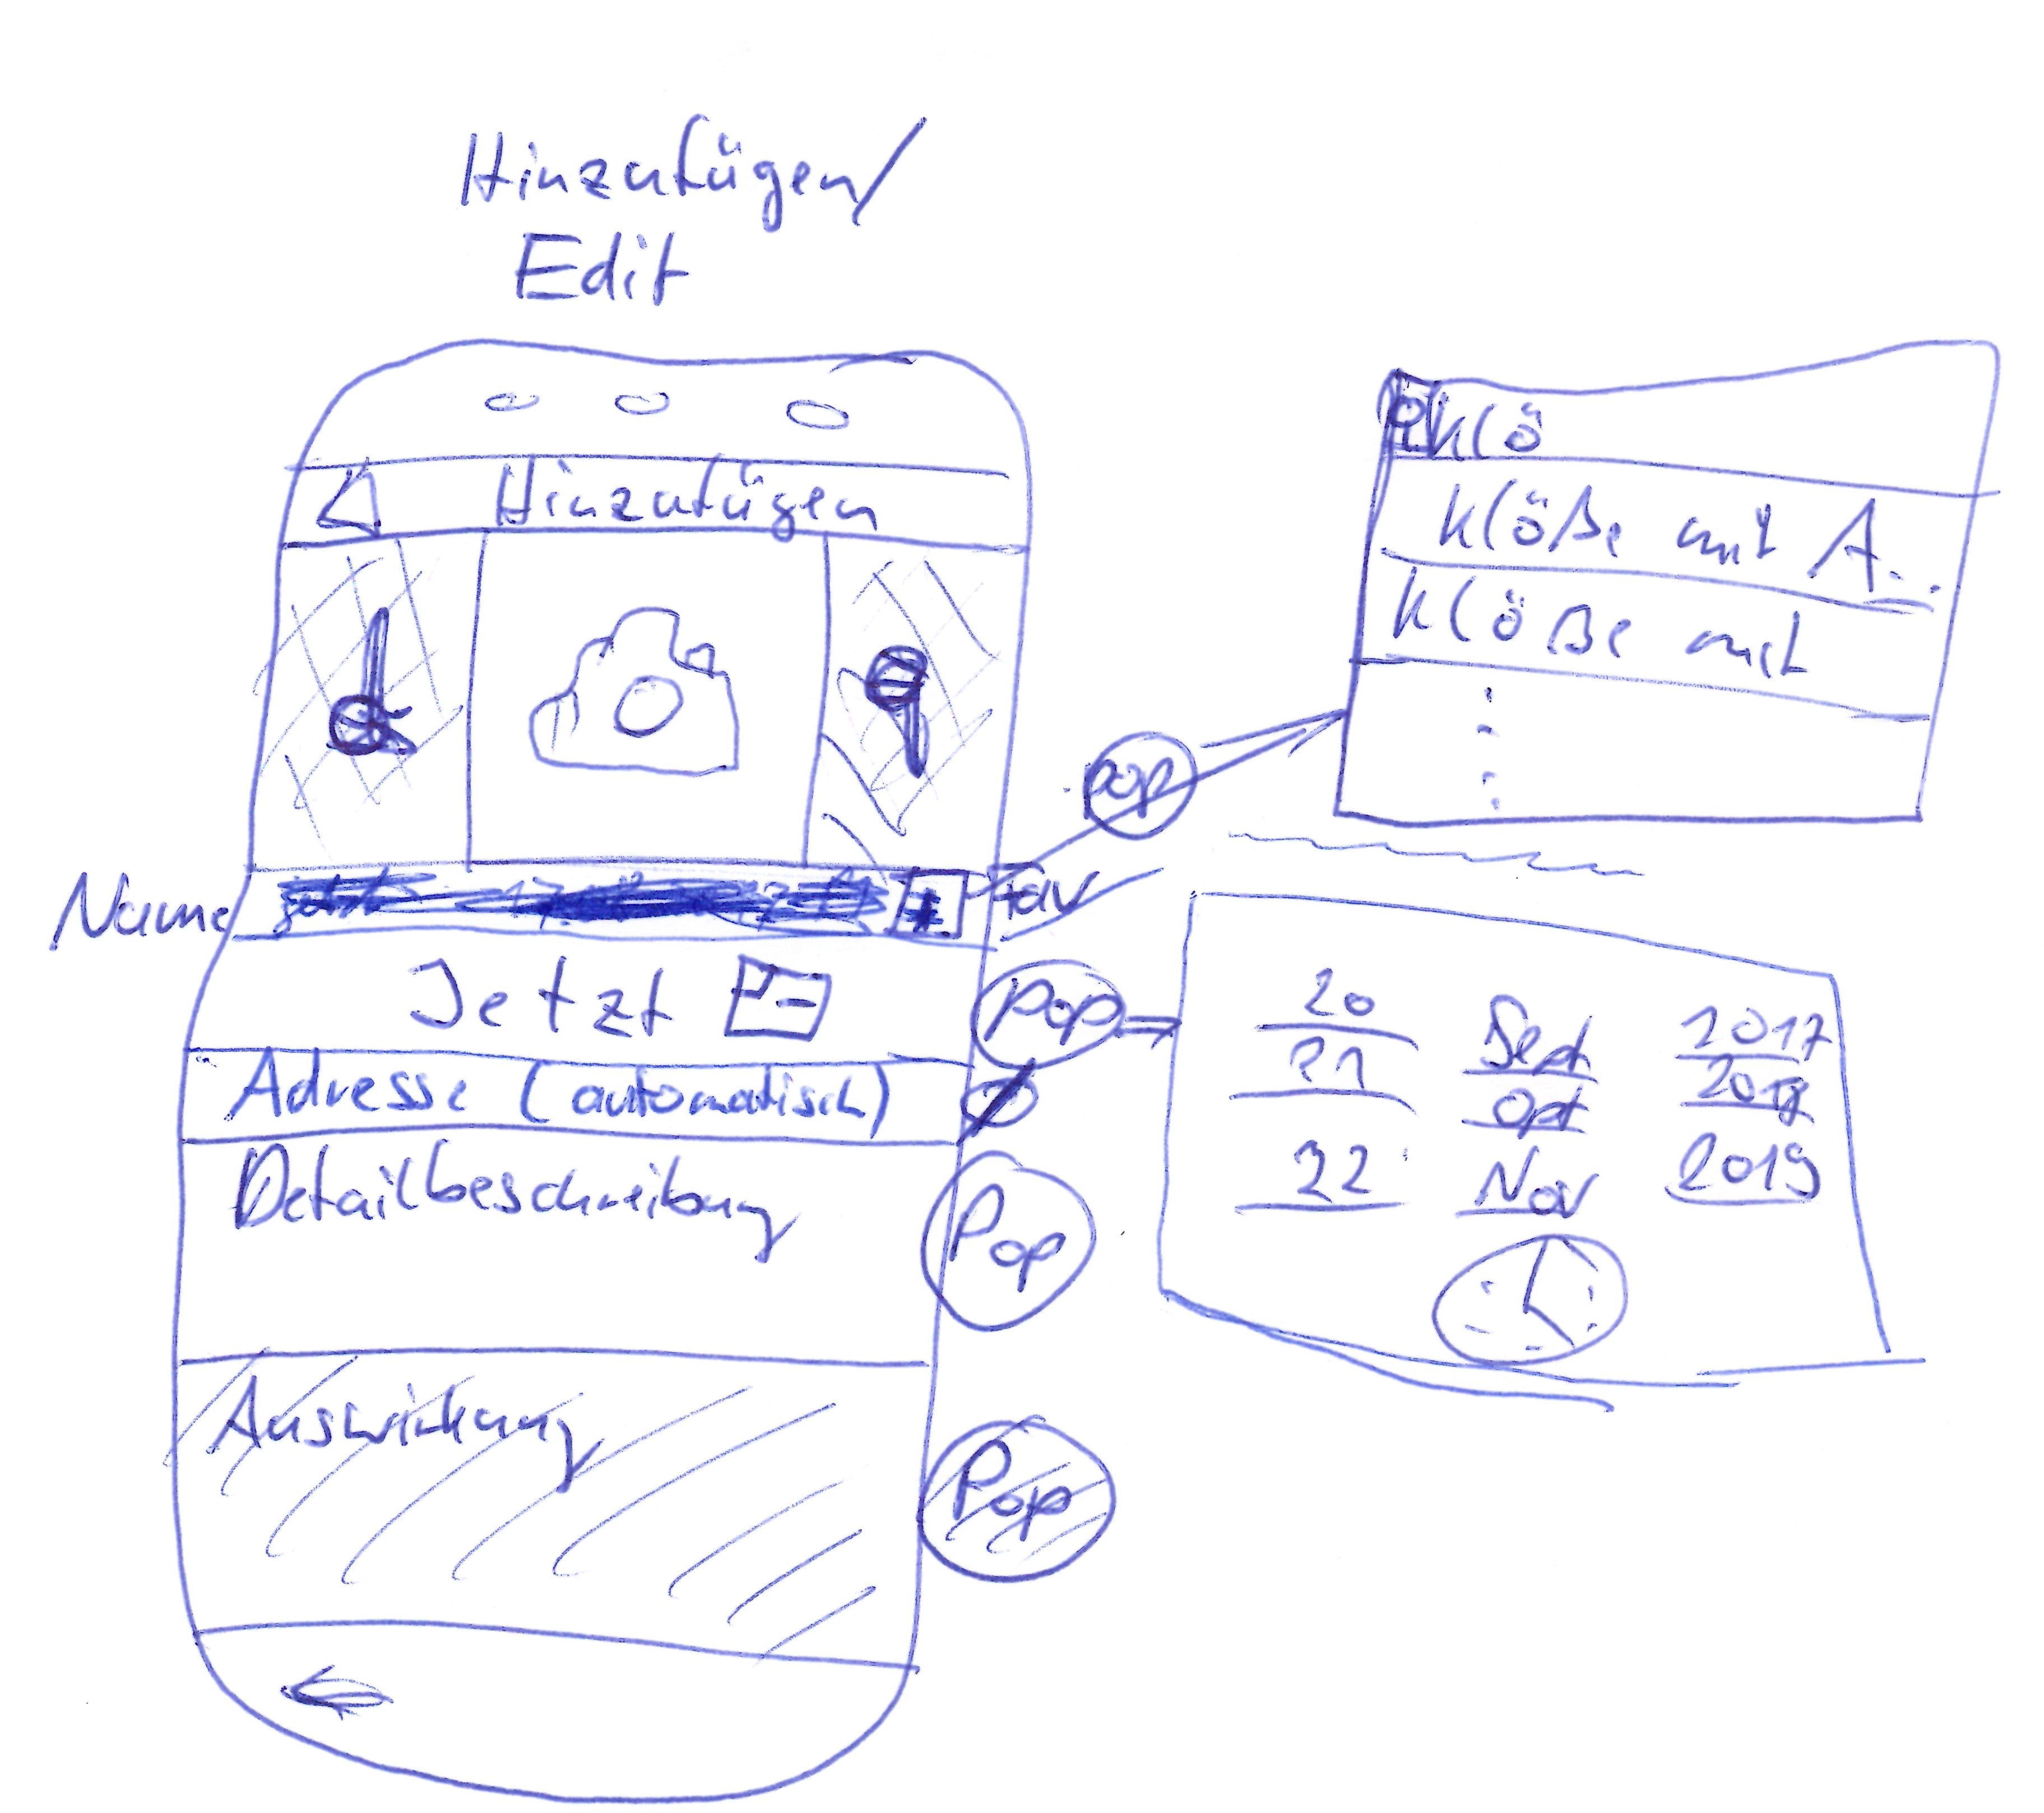
\includegraphics[width=1.0\textwidth]{add_entwurf} }
	\caption{Hinzufügen eines Eintrags}
	\label{fig1}
\end{figure}


\begin{figure}[ht]
	\centering
  \frame{ 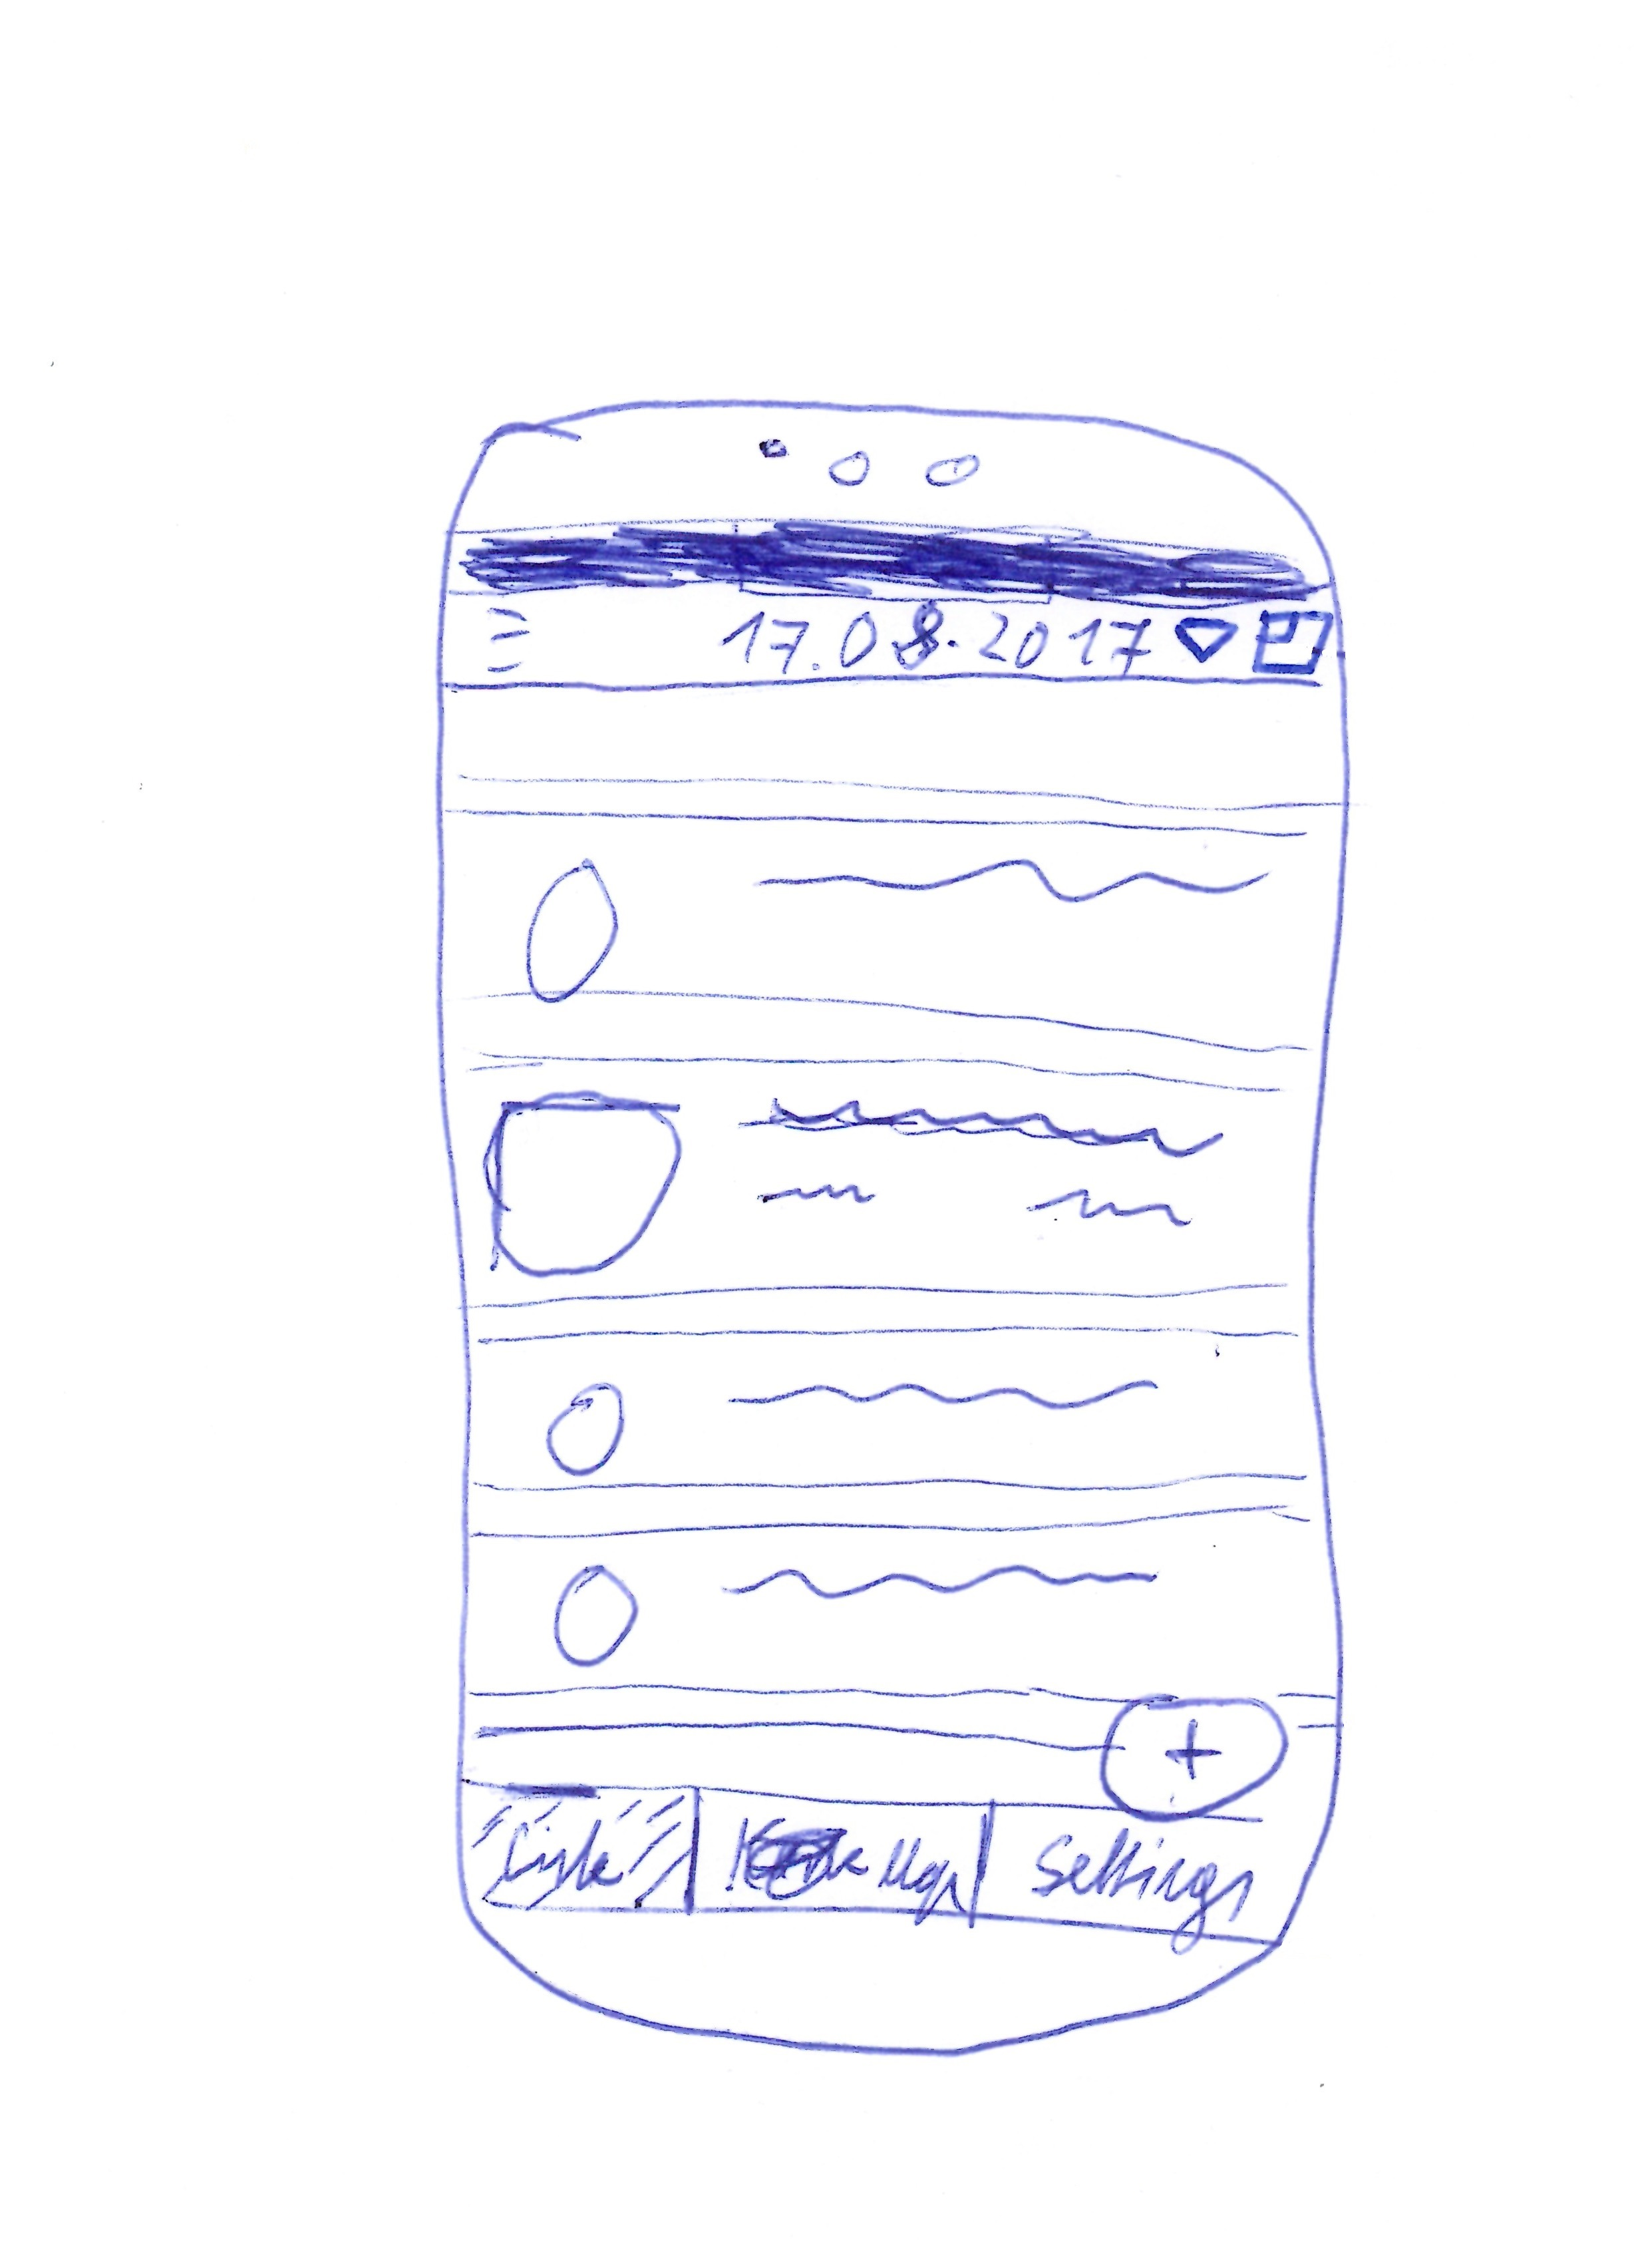
\includegraphics[width=1.0\textwidth]{main} }
	\caption{Main Screen}
	\label{fig1}
\end{figure}



\begin{figure}[ht]
	\centering
  \frame{ 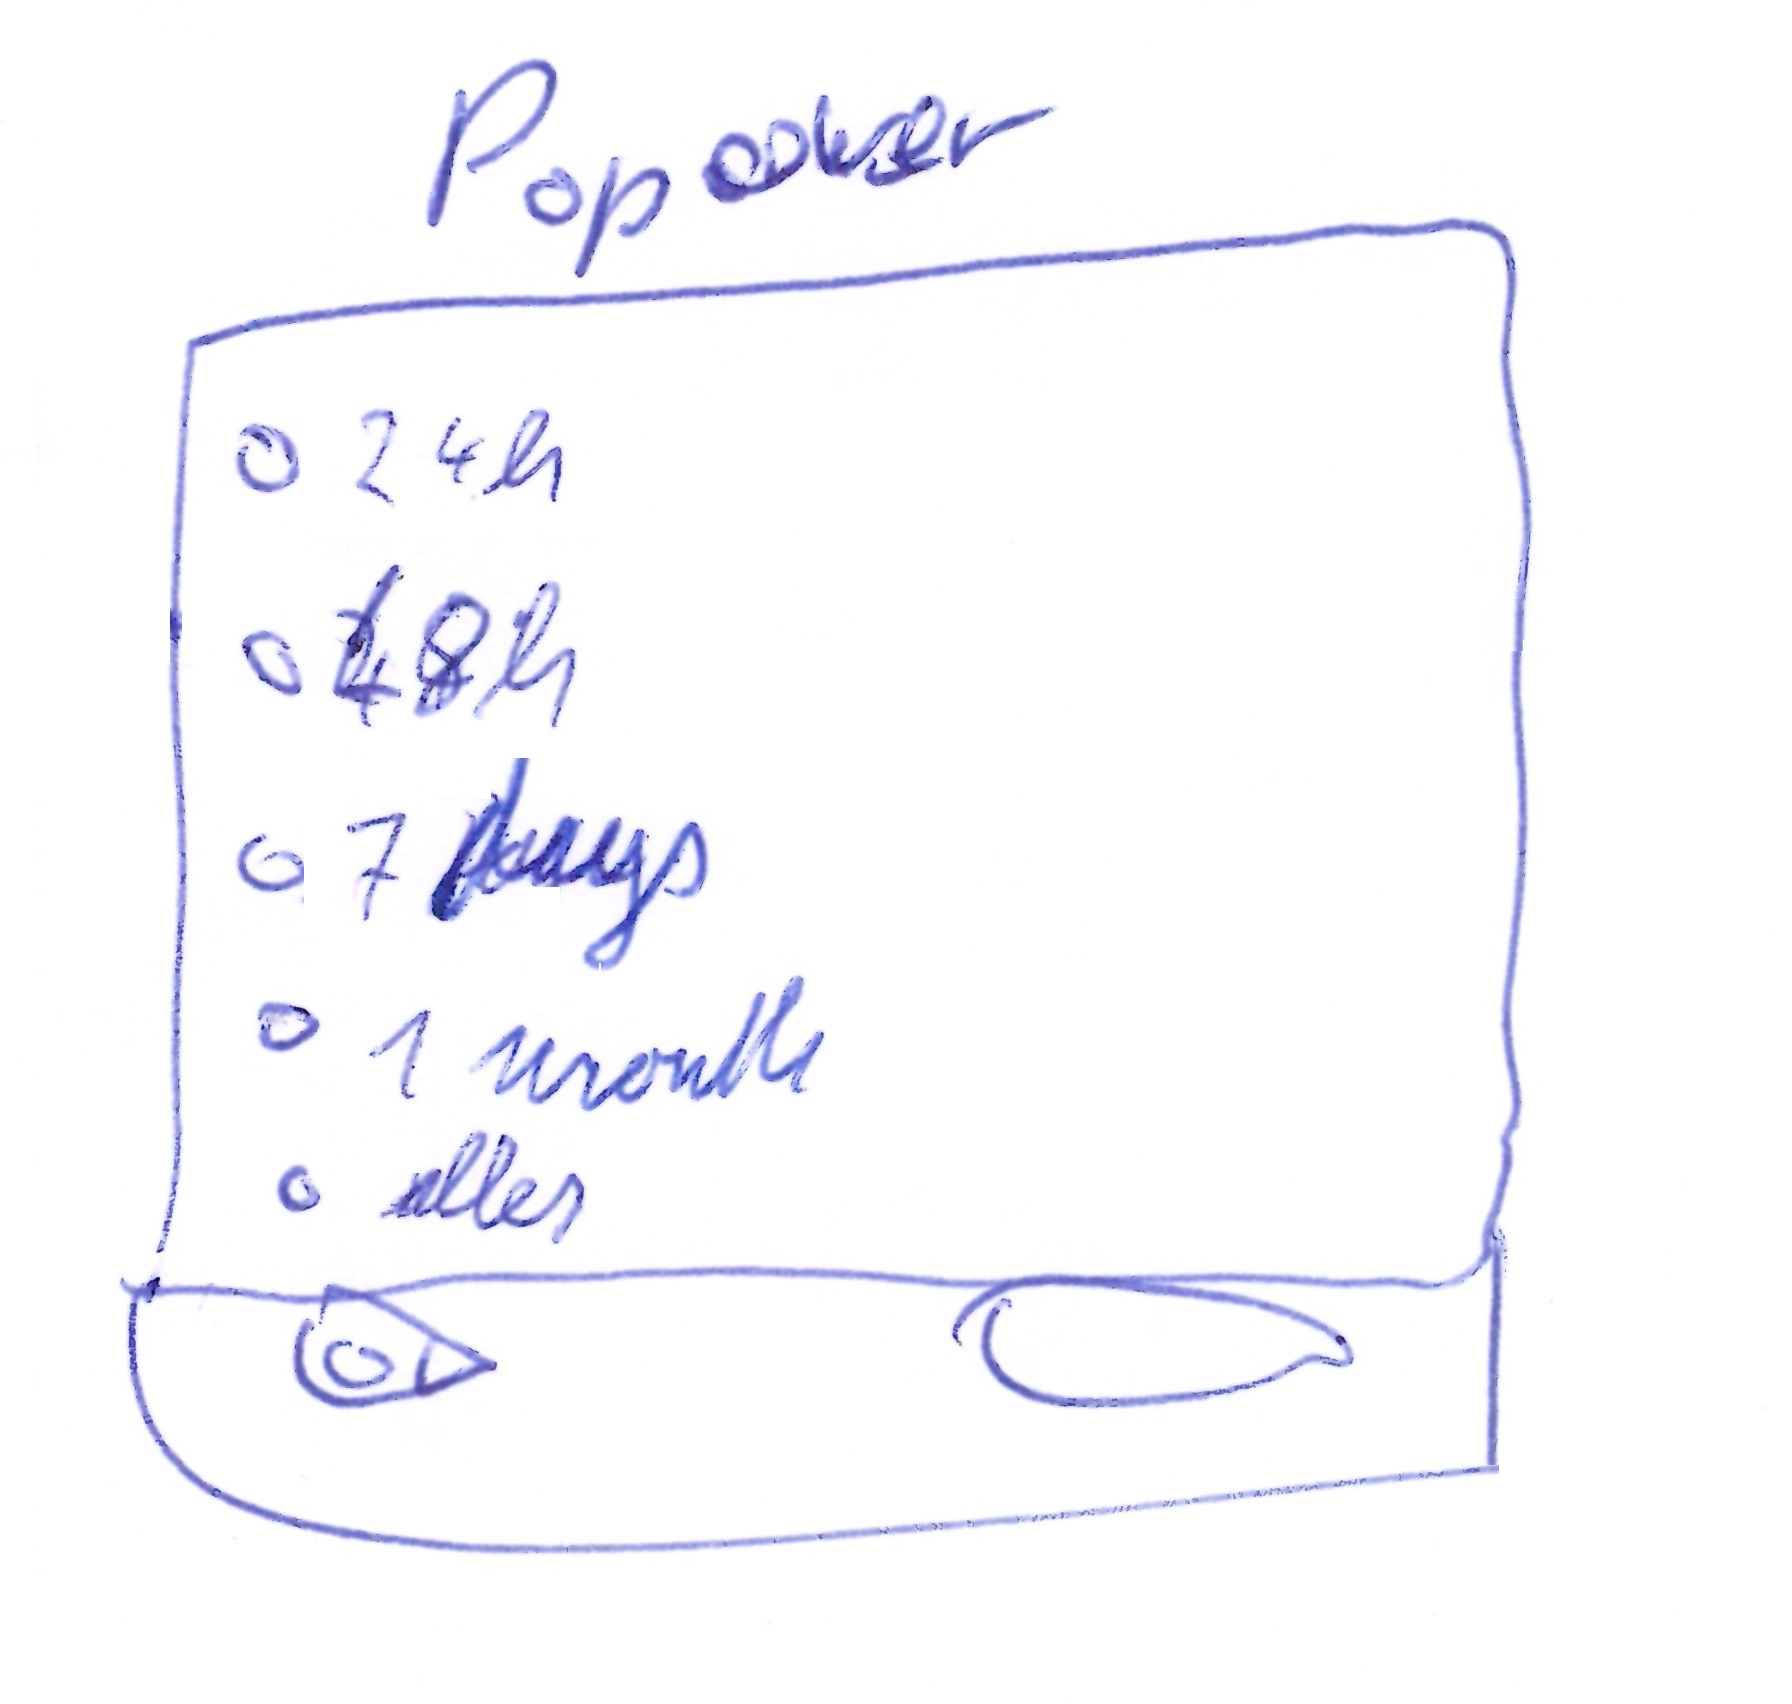
\includegraphics[width=1.0\textwidth]{popover} }
	\caption{Popover Screen}
	\label{fig1}
\end{figure}



\begin{figure}[ht]
	\centering
  \frame{ 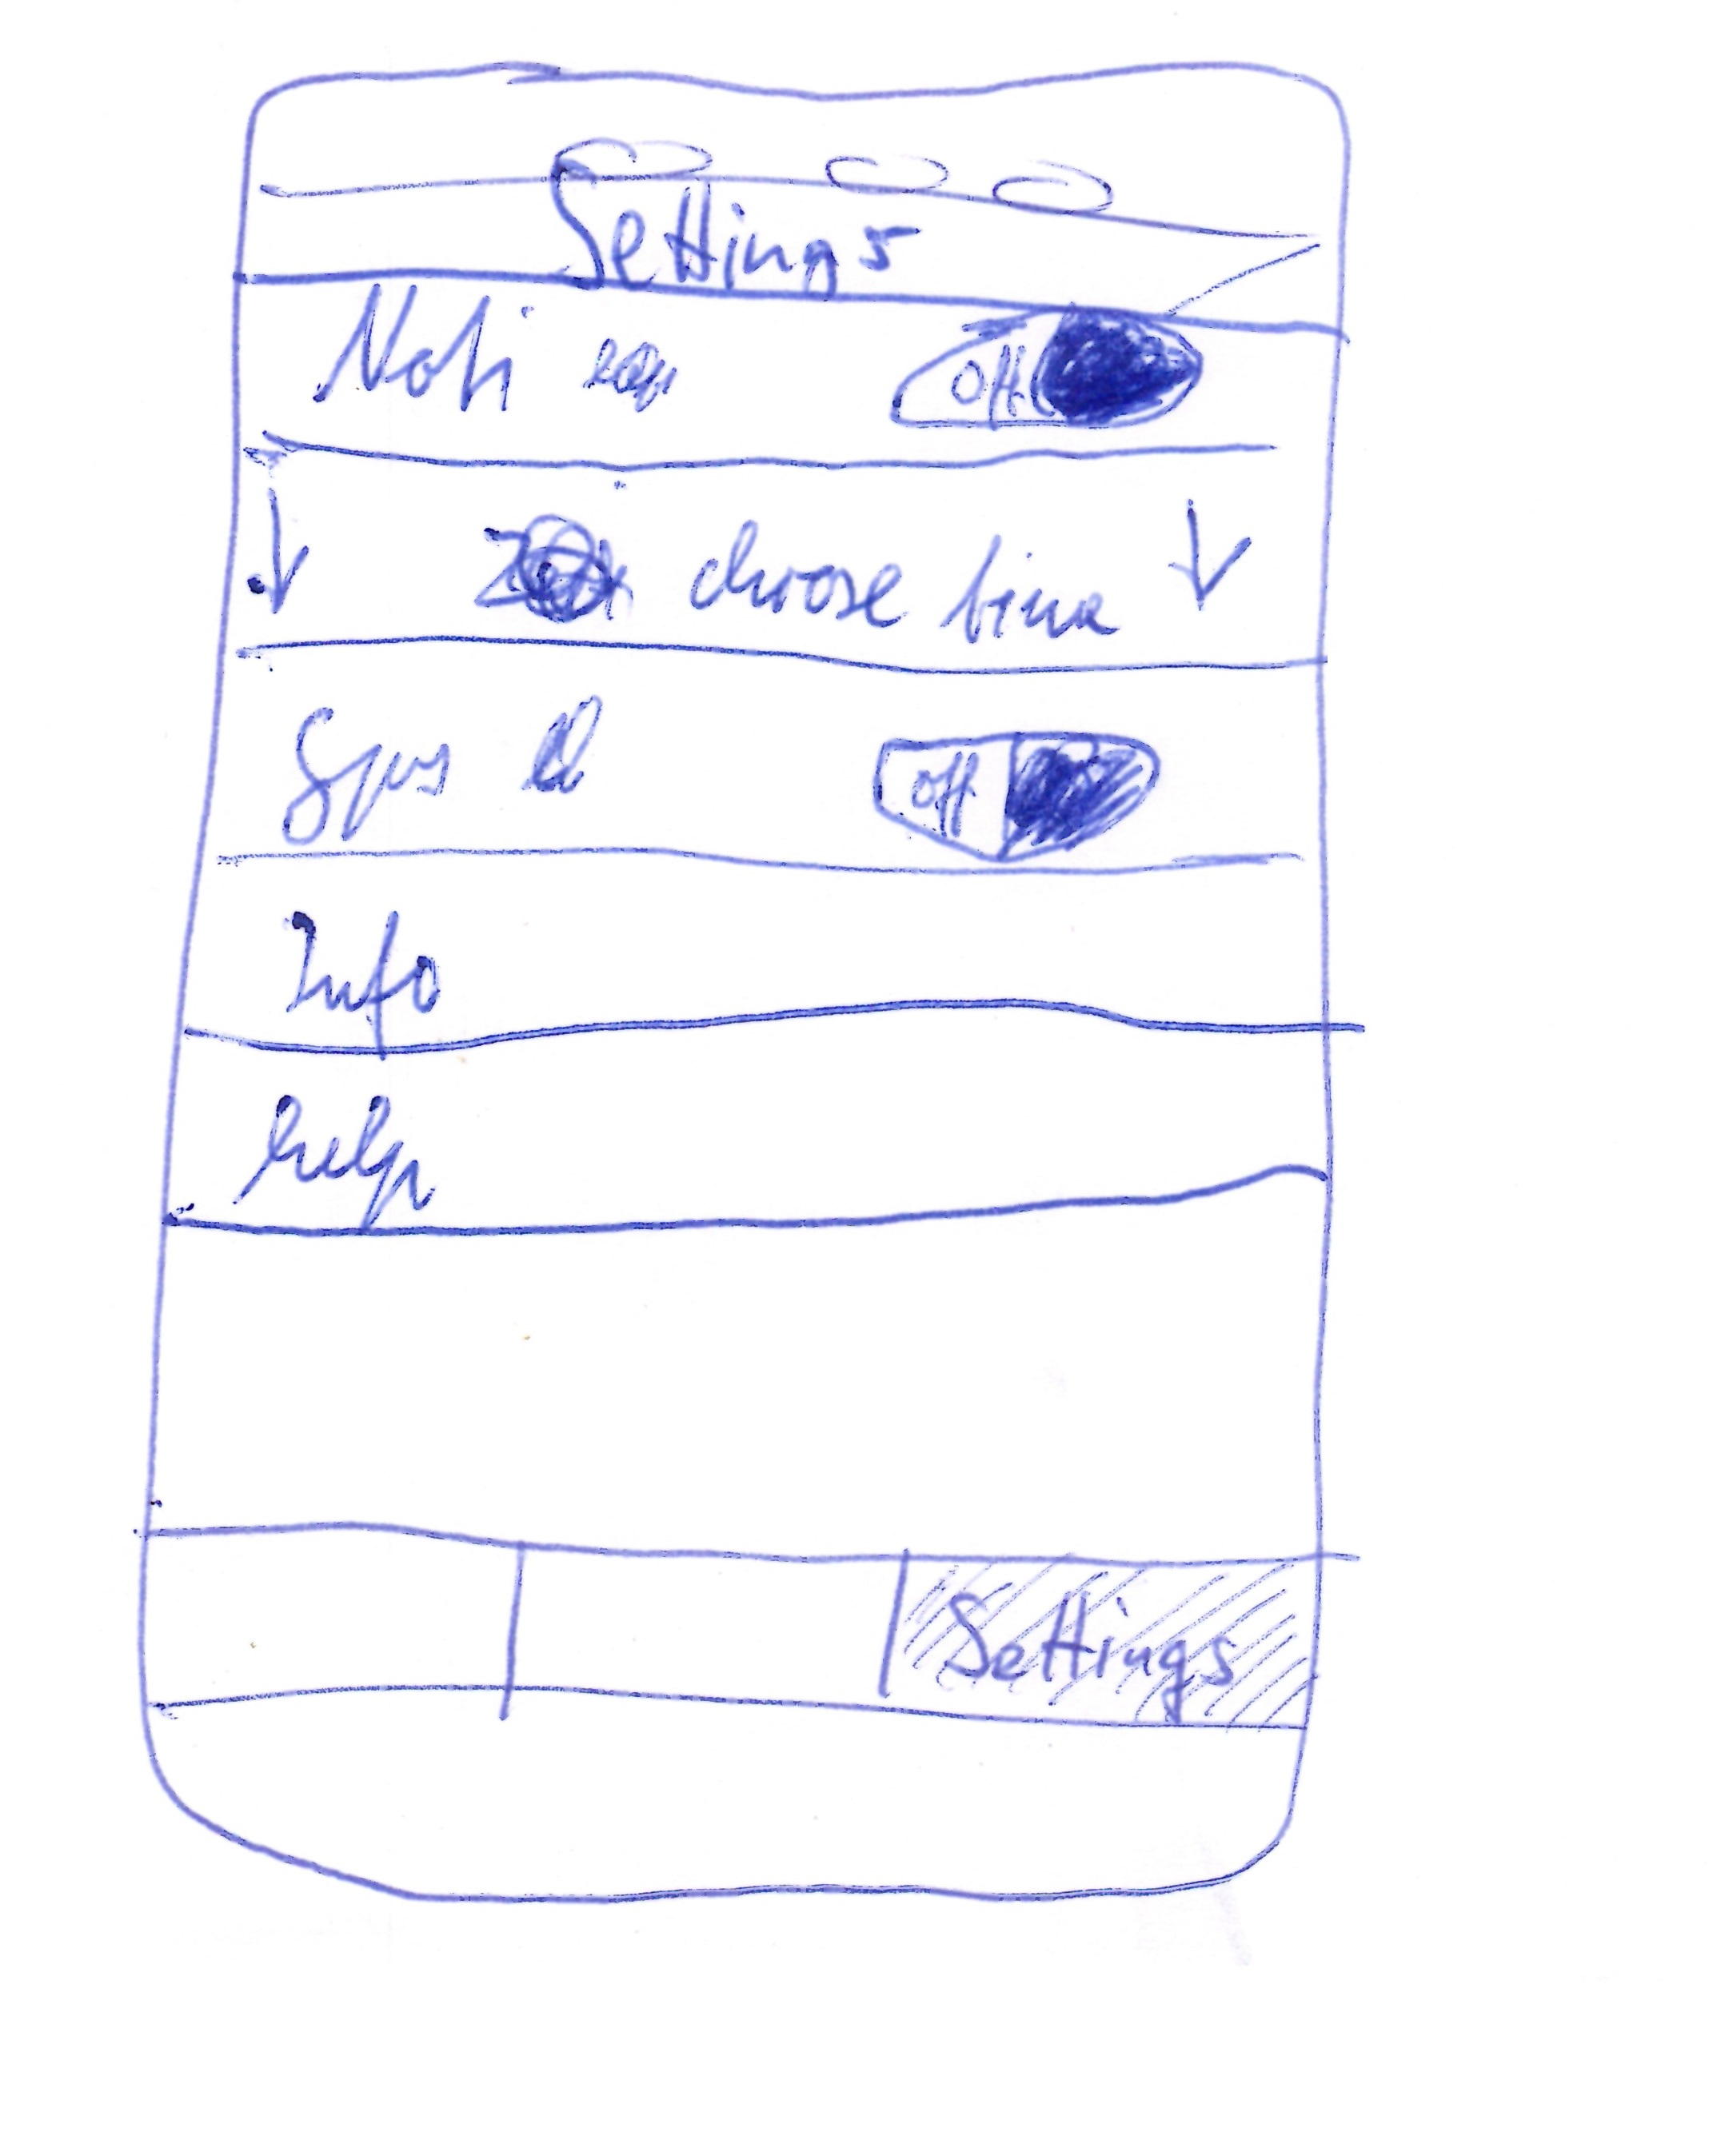
\includegraphics[width=1.0\textwidth]{settings} }
	\caption{Settings Screen}
	\label{fig1}
\end{figure}





\begin{figure}[ht]
	\centering
  \frame{ 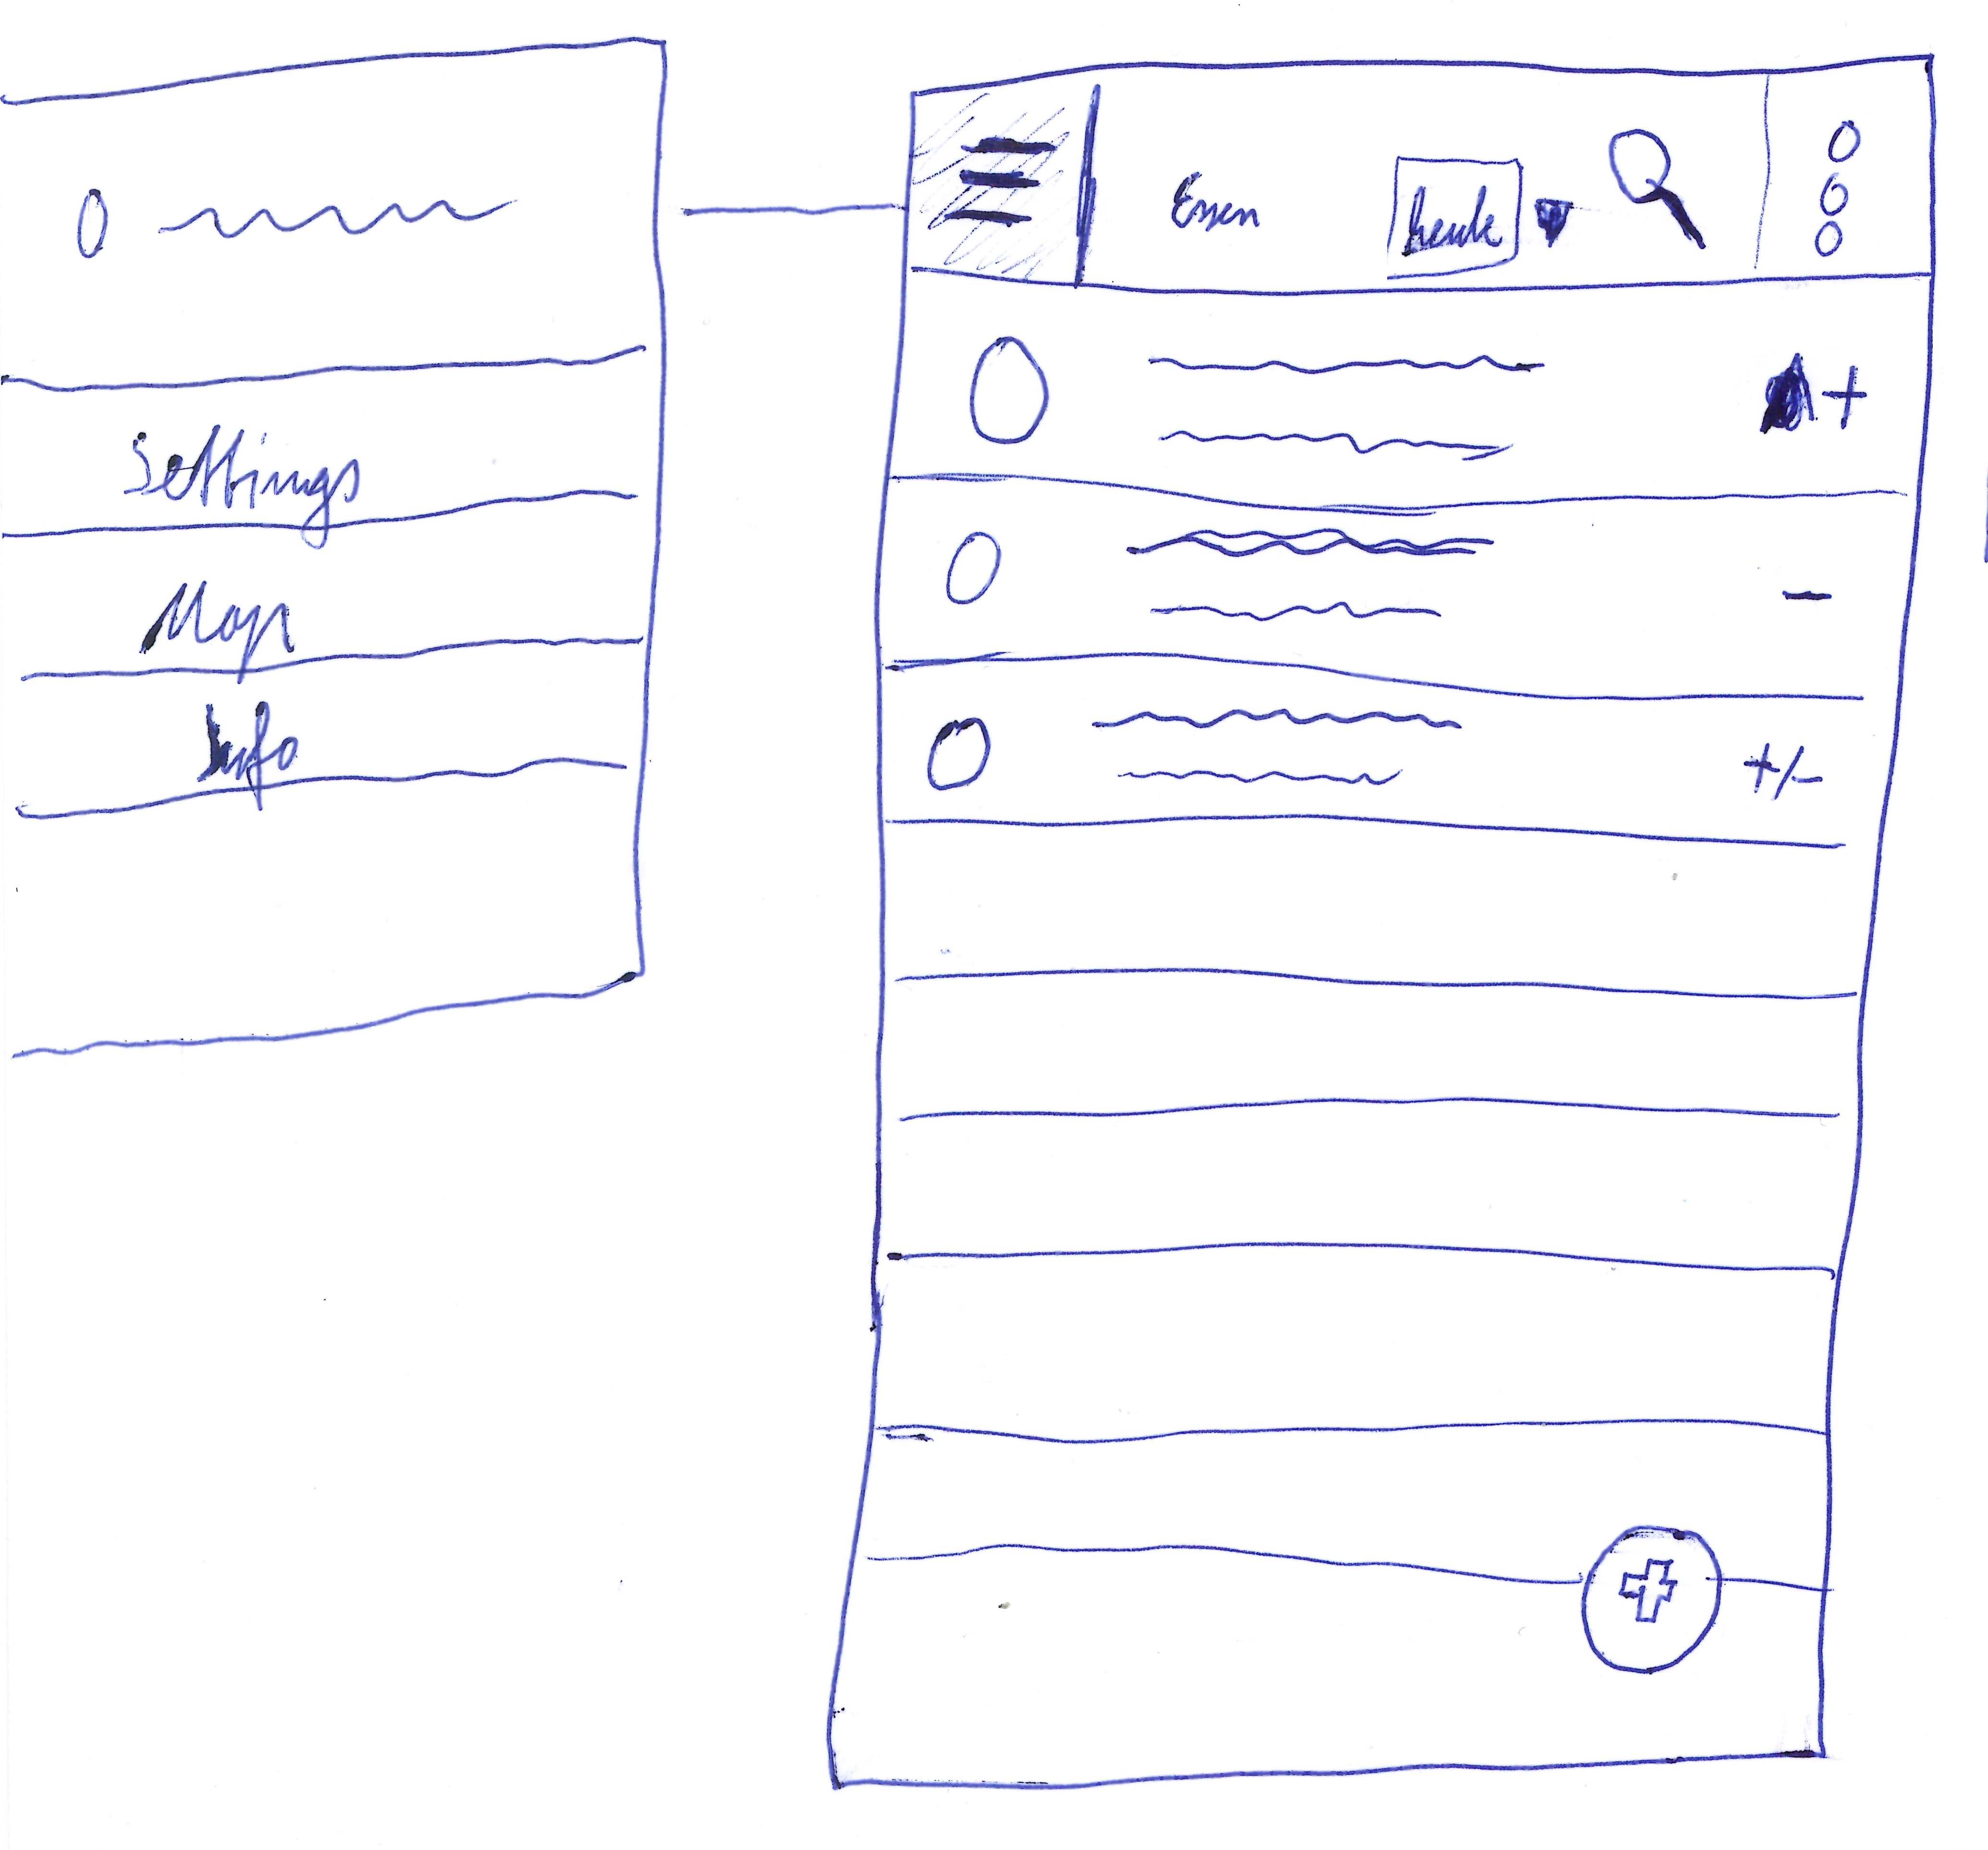
\includegraphics[width=1.0\textwidth]{main_burger} }
	\caption{Main Hamburger Menü Screen}
	\label{fig1}
\end{figure}







\newpage

\chapter{Umsetzung}

\newpage

\chapter{Aufgetretene Probleme}

\newpage

\chapter{Lessons learned}



\newpage

\chapter{Weitere Arbeiten}
In diesem Projektabschnitt konnten alle gesteckten Ziele erreicht werden. Da solch ein junges Projekt noch viele Möglichkeiten beinhaltet Funktionen zu verbessern und neue Funktionen einzuführen werden hier mögliche Punkte zur Anregung aufgelistet.
\newpage


\listoffigures

\end{document}